\documentclass{TDP005mall}



\newcommand{\version}{Version 1.0}
\author{Love Jansson, \url{lovja643@student.liu.se}\\
  Charlie Simonsson, \url{chasi127@student.liu.se}}
  
\title{Kravspecifikation - Comet Raids}
\date{2019-11-26}
\rhead{Love Jansson \\ Charlie Simonsson}
\usepackage[final]{pdfpages}



\begin{document}
\projectpage
\section{Revisionshistorik}
\begin{table}[!h]
\begin{tabularx}{\linewidth}{|l|X|l|}
\hline
Ver. & Revisionsbeskrivning & Datum \\\hline
0.1 & Dokument kopierad från mall & 191115 \\\hline
0.5 & Första utkast & 191120\\\hline
1.0 & Kravspecifikationen klar för inskick.& 191126\\\hline



\end{tabularx}
\end{table}

\tableofcontents
\pagebreak 

\section{Inledning}
Denna kravspecifikation avser ett objektorienterat projekt i form av ett två 
dimensionellt arkadspel. Spelet kommer ha ett rymdtema och målet är att i en 
rymdfarkost navigera en bana med olika faror för att placera ut bomber på 
förutbestämda platser. I resterande del av dokumentet presenteras en utförligare
beskrivning av spelet samt vilka krav slutprodukten ska uppfylla. Bomber
isblock projektiler och skepp refereras till kollektivt som objekt eller
objektet i singular.

\section{Spelidé}
Jorden är i fara!\\
Ett moln av stora kometer närmar sig jorden från solsystemets utkant och det är 
spelarens uppgift att förstöra dessa. Detta sker genom nogrann placering av 
bomber inuti kometerna. På vägen måste spelaren överkomma lokala faror bestående
av svävande isblock av varierande storlek genom att skjuta sönder dem.
I spelet representeras varje komet av en bana och spelaren måste lösa varje 
bana för att jorden ska vara säker igen. 

\subsection{Spelets mål}
Det övergripande målet är att förstöra alla kometer. I varje komet finns 
specifika delmål:\\
1. Spelaren ska placera ut bomber på samtliga angivna platser.\\
2. Från och med att första bomben har placerats har spelaren ett begränsat antal
sekunder på sig att lämna kometen innan den sprängs.\\
3. Samtidigt som ovanstående mål uppfylls måste spelaren  skydda sig mot de
svävande isblocken genom att skjuta dem eller undvika dem.



\subsection{Spelmekanik}
Spelet spelas antingen i singleplayer(ska-krav) eller i two player(bör-krav) där
spelarna delar på tangentbordet. 
En spelare behöver 6 tangenter för att styra rymdskeppet, en tangent som styr
skjutvapnet och en tangent som reglerar den annordning som finns för att släppa
bomber. Se nedanstående
uppställning angående vilka tangenter som kommer användas. 

\begin{table}[!h]
\begin{tabularx}{\linewidth}{|X|l|l|}
\hline  
Kommandon  & Player 1 & Player 2 \\\hline
Framåt i skeppets riktning: & w & num-pad 8 \\\hline
Bakåt i skeppets riktning: & s & num-pad 2 \\\hline
Vänster i skeppets riktning: & a & num-pad 4 \\\hline
Höger i skeppets riktning: & d & num-pad 6 \\\hline
Rotera vänster: & q & num-pad 7 \\\hline
Rotera höger: & e & num-pad 9 \\\hline
Kanon: & space & piltangent ned \\\hline
Bomb: & b & num-pad 0 \\\hline

\end{tabularx}
\end{table}
Tabell 1: Översikt av tangenter för spelare 1 och spelare 2.

\textbf{Spelets fysiska regler}
Spelets fysik är en simulation av Newtons fysiska lagar. 
Detta innebär att vi kommer simulera microgravitation, dvs. ett objekt förblir i
vila eller i likformig rörelse om inga andra krafter påverkar det.

Kartan kommer vara statisk. Det kommer finnas objekt renderade på skärmen som
rör sig. Det är enbart spelarobjektet (farkosten) som kan påverka sig självt och
övriga objekt kommer enbart röra sig om de påverkas av en spelare direkt, tex. 
genom att spelaren skjuter på objektet eller spelaren medvetet rammar objektet,
eller indirekt via andra objekt (kollisioner).

\textbf{HP och kollisioner}
Varje objekt av typen isblock och farkost har liv vilket representeras som 
HP -eng. Hit Point(s)-. Farkosten ska dessutom ha en sköld som även den har HP.
När skölden når noll kommer skeppet ta HP skada och riskera att förstöras.

De objekt som spelet består av kan kollidera och ta skada på olika sätt.\\
Kollisioner mellan isblock ska vara ickeelastiska dvs., de ska slås samman och
ges en riktning och hastighet som beräknas från de samanslagna blockens dito.

Block vars HP når noll ska de delas upp i mindre delar på följande vis:
2 st block med storleken: (tidigareblocks storlek/2) 
samt ett block med nya storleken: 1 * resten av (tidigareblocks storlek / 2) 
om nya storleken är större än noll.

Vid skapandet av nya isblock i samband med splittring ska de nya isblockens
riktning och hastighet bestämmas som en funktion på ursprungliga isblockets
riktning och hastighet adderad till en randomiserad normaliserad vector. 

Detta beskrivs mer utförligt under avsnitt 'Kravforumlering'.
Farkostens kollisioner är elastiska dvs., den studsar med de objekt den
kolliderar med, förutsatt att farkostens HP inte når noll av den skada den tar
vid kollisionen. \\

I mån av tid kommer projektiler inplementeras. Dessa skjuts från farkostens kanon
och gör skada vid kollisioner. Efter kollision försvinner projektilen.

\textbf{Bomb}
Bomber har två beteenden.
1. Om en bomb placeras inom utsatt bombzon startas en tidsräkning och bomben blir
statiskt placerad dvs., det kommer inte gå att flytta eller skada den.

2. I alla andra fall kommer bomben fortsätta att färdas i  den hastighet och 
riktning som den skapades med tills den träffar en bombzon då den byter till 
tillstånd 1(se ovan). Om bomben kolliderar med väggar eller objekt innan 
den når en bombzon exploderar den och gör skada på allt inom räckvidden. Undantag:
En bomb i detta tillstånd som träffas av en projektil ska förstöras utan detonation.

\subsection{Regler}
Spelaren klarar av en bana genom att placera bomber på alla angivna platser samt
lämna kometen innan nedräkningen på den först placerade bomben har löpt ut.
Spelaren har möjligheten att placera bomber på andra ställen också, men hen
måste tänka på att antalet bomber är begränsat och därmed planera spelgången mer
noggrant. I fall two player utvecklas för spelet räcker det att en spelare
lyckas med ovan dvs., banan är avklarad även om en farkost kraschar. När alla
banor är avklarade är jorden fri från hotet av kometer.

Banorna(kometerna) blir succesivt svårare att spränga desto fler banor(kometer)
som sprängs. Svårighetsgraden baseras på antal bombplatser och komplexitet av
layout. Layoutens komplexitet beror på hur trånga gångar som finns samt hur
många svängar spelaren måste navigera för att ta sig fram i banan.

När farkosten kolliderar med isblock, väggar, projektiler och bomber, kommer den
ta skada. Detta beskrivs mer utförligt under Spelmeknik rubriken.

Spelet förloras antingen om farkosten tar så mycket skada att HP
går ned till 0 alternativt om en av de bomber som är placerade på avsedda zoner
detonerar innan övriga vinstkriterier är uppfyllda.  

\pagebreak

\subsection{Visualisering}
När spelet först startas så presenteras spelaren med en meny med valet att
starta spelet eller avsluta spelet.

Spelet utspelar sig i tunnlar inuti en komet sätt ovanifrån. Väggarna är is och
ska ha olika nyanser av blå färg. Tunnlarna  har svart bakgrund för att spelare
ska kunna se vad som händer i spelet. I tunnlarna finns även lösa isblock vilka
ska ha samma färg som väggarna. Spelarna ska ta sig förbi dessa för att komma
fram till de zoner där bomber ska placeras. Dessa zoner är kometens svaga
punkter och de är markerade med röda ringar. Bilden nedan visar ett exempel på
hur det kan se ut inuti en komet.

I mån av tid kommer spelet ha ett lager som ligger över banan som döljer de
områden som spelaren inte besökt. Detta refereras till generellt som Fog-of-War.
Genom att göra detta lager genomskinligt innom en viss radie från spelaren kan
banan utforskas. Detta ökar spänningen en spelare upplever och gör banans
faror mer påträngande. I samband med denna utökning planeras det att lägga till 
en minikarta i något av spelfönstrets övre hörn i syfte att ge spelaren ledning
om var hen är på banan.

\begin{figure}[h!]
\caption{Bana med farkost, isblock, svaga punkter och bomb.}
\includegraphics[scale=0.11]{../bilder/Bana1.pdf}
\end{figure}

\begin{figure}[h!]
  \caption{Farkost.}
  \center
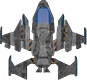
\includegraphics[scale=1.5]{../bilder/Ship/ship0.png}
\end{figure}

\begin{figure}[h!]
  \caption{Isblock i olika storlekar.}
    \center
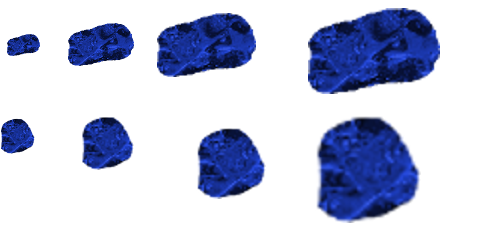
\includegraphics[scale=0.2]{../bilder/originals/Ice_Blocks.png}
\end{figure}

\begin{figure}[h!]
  \caption{Bomb.}
  \center

\includegraphics[scale=1.0]{../bilder/originals/bomb.png}
\end{figure}

\begin{figure}[h!]
\caption{Bomb explosion.}
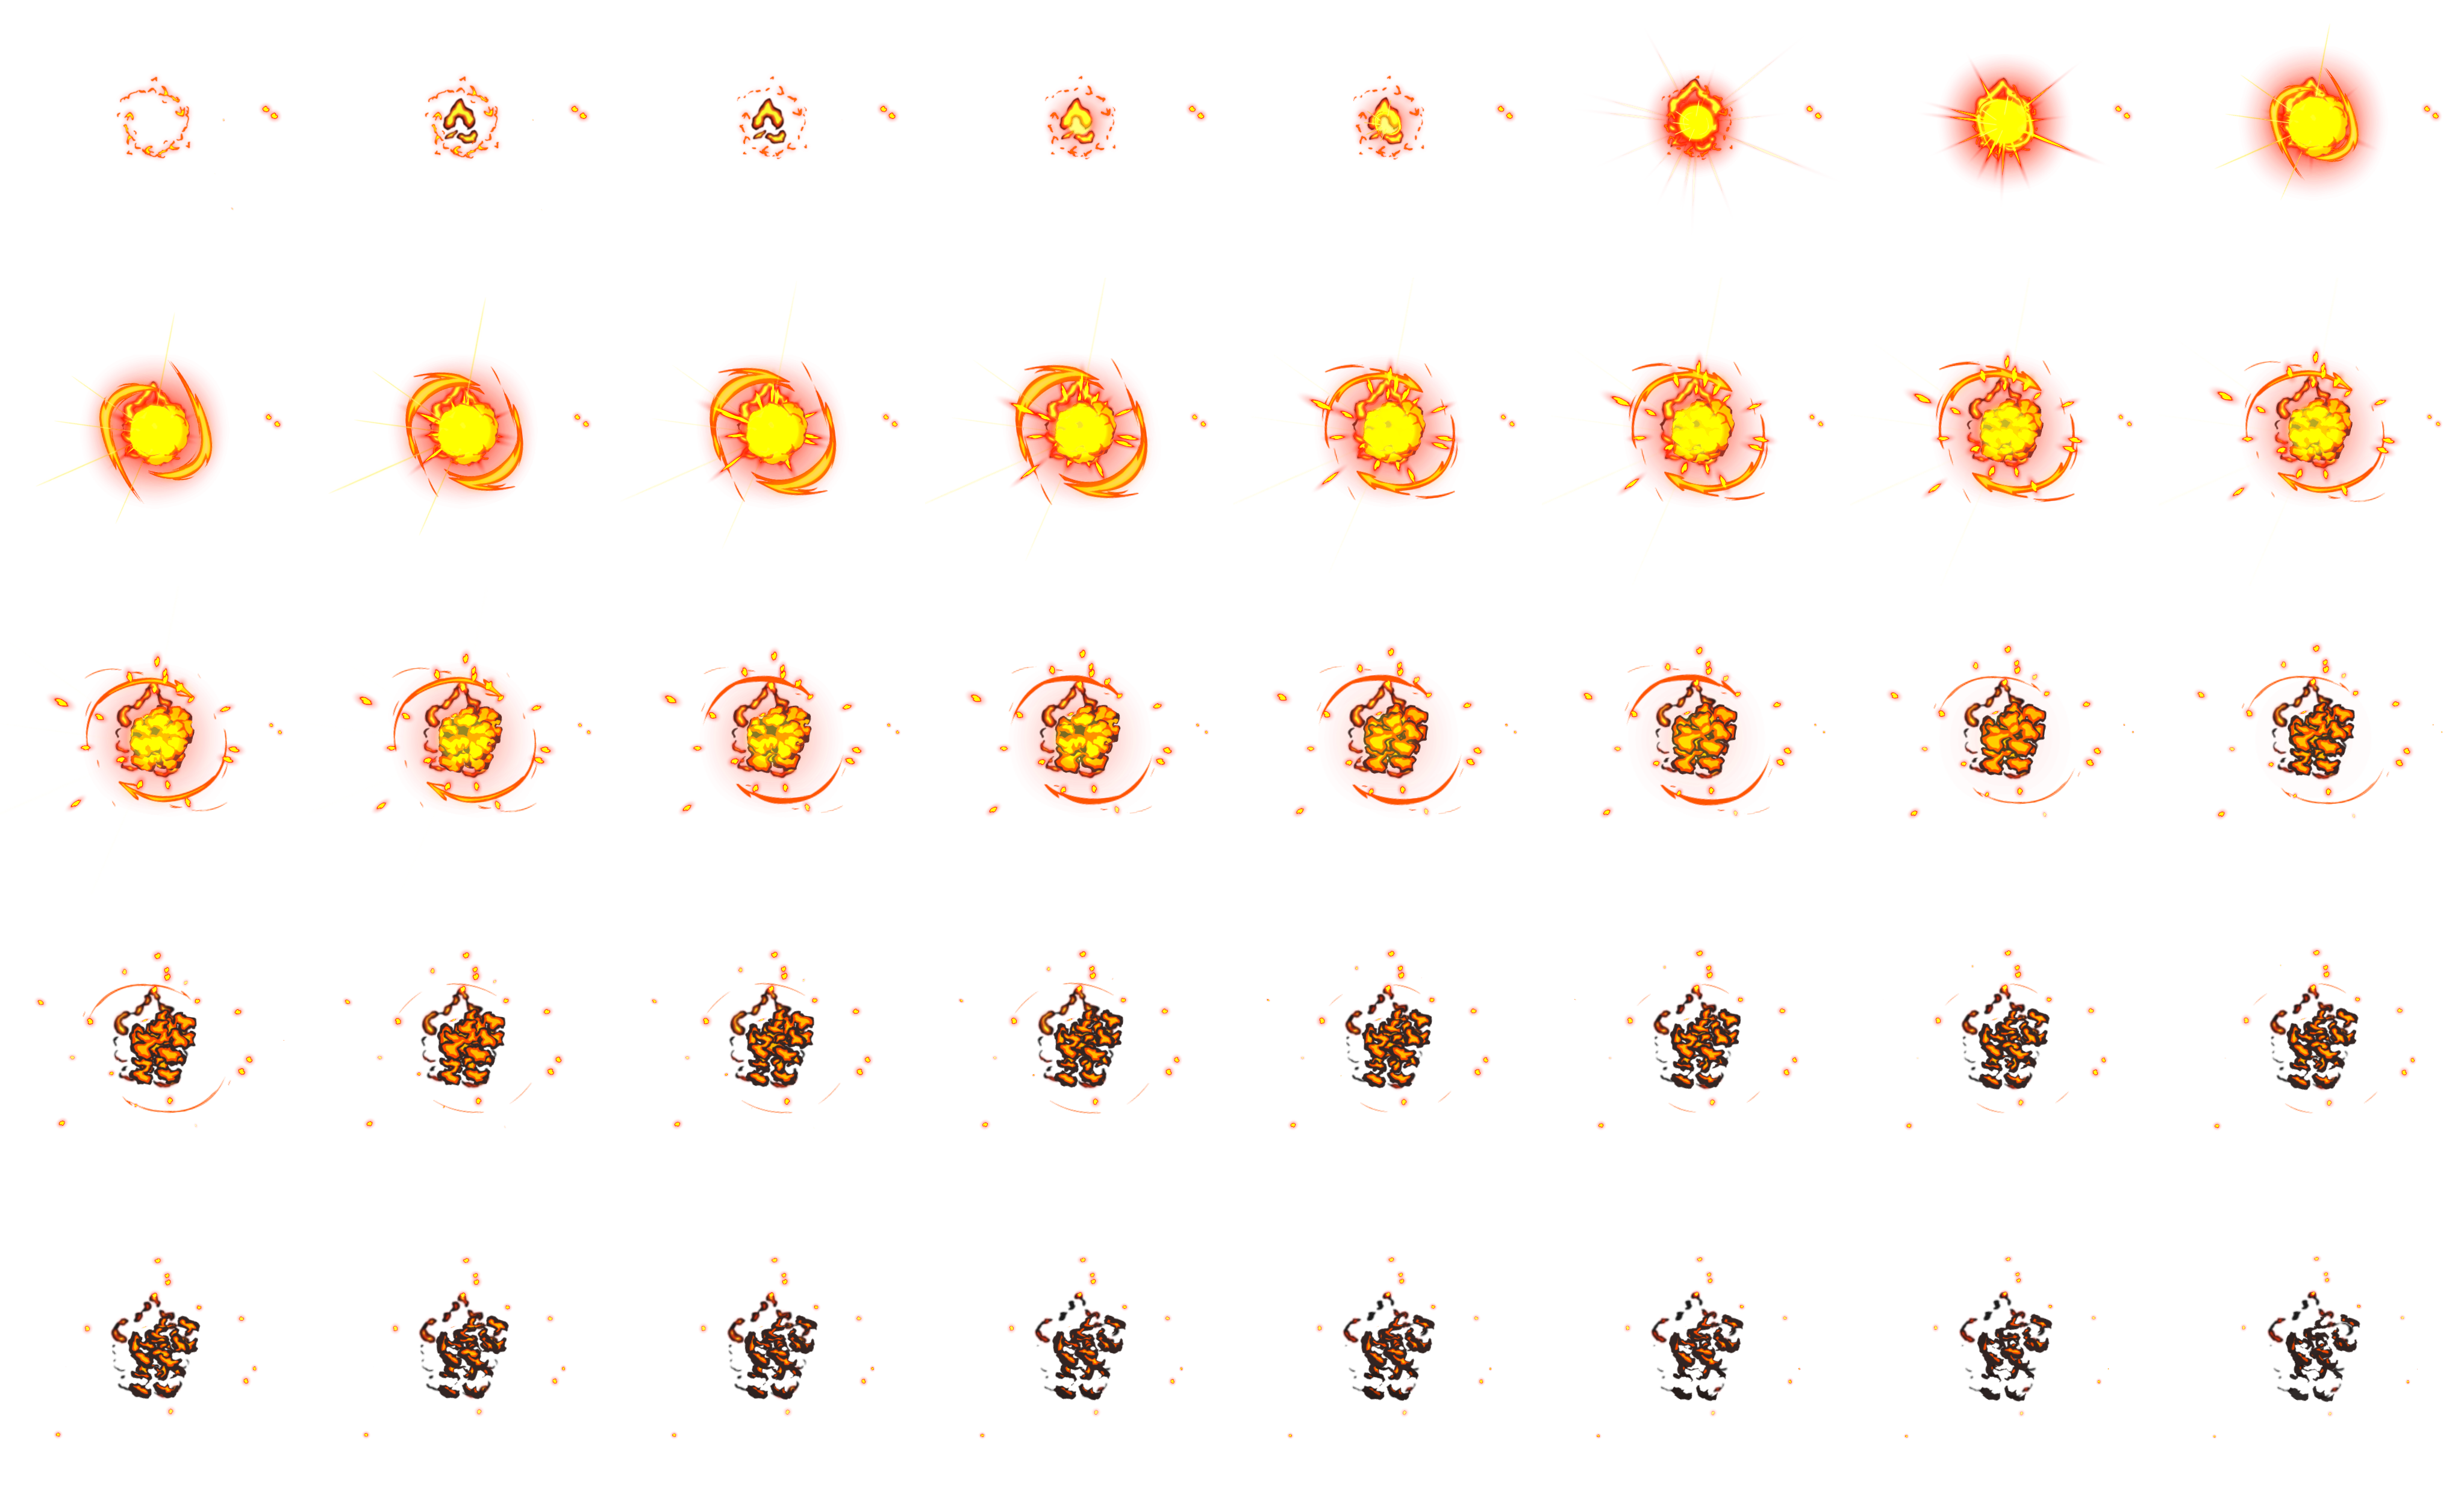
\includegraphics[scale=0.11]{../bilder/explosions/explosion_4.png}
\end{figure}
\pagebreak  

\subsection{Spelupplevelse}
Spelet kommer kräva planering, timing, samarbete (om det är två spelare som
spelar) och tålamod.\\
Med detta spel försöker vi fånga en 'old school feeling' i form av ett arkadspel
som kräver tid och dedikation för att bli bra. Spelet kommer ta spelaren
tillbaka till tiden då 'Highscore' betydde något.

\subsection{Målgrupp}
Vår målgrupp är dator spelare som gillar utmaningar. Spelaren stimuleras av
tidvis frustrerande spelmoment där spelarens egen oaktsamhet får drastiska
konsekvenser för spelets svårighetsgrad. 
\pagebreak

\section{Kravformulering}
Nedan beskrivs de krav som ställs på projektet. Kraven delas upp i två grupper:
ska-krav och bör-krav. Ska-kraven måste uppfyllas för att projektet ska anses
vara godkänt. I mån om tid implementeras bör-kraven i tur och ordning.

\subsection{Ska-krav}

\textbf{Almänna Krav}\\
0.1 Språket i spelet ska vara svenska. \\
0.2 Spelet ska kunnas spelas i single player läge. \\

\textbf{Banan}\\
1.1 Spelet ska simulera mikrogravitaion i 2 dimensioner inuti en komet, se
spelmekaniska regler. \\
1.2 Banan ska representeras av ett skal av väggar, se figur 1. \\
1.3 Det ska vara möjligt att läsa in fler banor pixelvis från bild. \\
1.4 Banan ska vara lika stor som fönstret.\\

\textbf{Farkosten}\\
2.1 Farkosten ska kunna styras i 2 dimensioner samt rotera 360 grader kring 
z-axeln, se tabell1. \\
2.2.1 Farkosten ska kunna släppa bomber i kometen. \\
2.2.2 Farkosten ska ha ett begränsat antal bomber. \\
\textbf{Hur Farkosten tar skada} \\
2.3.1 Farkosten ska kunna ta skada genom att kollidera med väggar. \\
2.3.2 Farkosten ska kunna ta skada genom att kollidera med isblock. \\
2.3.3 Farkosten ska kunna skadas av bomber. \\
2.4 Farkosten ska ha hp som minskar när farkosten tar skada. \\

\textbf{Isblock} \\
3.1 Isblock ska kunna kollidera med varandra. \\
3.2 När isblock kolliderar ska de slås samman till ett isblock med en
sammanslagen storlek. \\ 
3.3 Sammanslagna isblock ska få ny hastighet och riktning.
Se spelmekaniska regler. \\
\textbf{Hur Isblocken tar skada}\\
3.4.1 Isblocken ska kunna ta skada av bomber. \\
3.4.2 Isblocken ska kunna ta skada av att kollidera med farkosten. \\
3.4.3 Isblocken ska kunna ta skada av att kollidera med väggar. \\
3.5.1 När isblocken tar skada ska de delas i mindre delar som har ny
hastighet och riktning, se spelmekaniska regler. \\
3.5.2 Isblock ska ha en minsta möjliga storlek. \\
3.5.3 När isblocken är av sin minsta möjliga storlek ska de kunna förstöras
helt vid skada. \\

\textbf{Bomber}\\
4.1 Bombernas hastighet och riktning ska vara lika med farkostens hastighet
och riktning när den släpps. \\
\textbf{Bombernas beteenden}\\
4.2 En bomb som släpps i en bombzon ska bli statisk och osårbar.\\
4.3 När den första bomben är placerad i en bombzon så startas en timer,
se spel regler.\\
4.4 En bomb som släpps utanför en bombzon ska kunna kollidera med objekt.\\
\textbf{Bombkollisioner}\\
4.5.1 En bomb som kolliderar ska explodera.\\
4.5.2 När en bomb exploderar ska bomben upphöra att existera. \\

\textbf{Förlust villkor} \\
5.1 Spelet ska avslutas om alla farkoster förstörs.\\
5.2 Spelet ska avslutas om end-timern löper ut och farkoster finns kvar i kometen.\\

\textbf{Vinst villkor} \\
6.1 En bana ska vara avklarad om bomber har placerats på alla avsedda platser
och farkosten har nått fram till banans slut.\\


\subsection{Bör-krav}
Nedan följer de krav vi vill göra i mån av tid. 

\textbf{Projektiler}\\
7.1 Projektiler som kolliderar med andra objekt ska försvinna. \\
7.2.1 Projektiler ska ha en konstant egen hastighet. \\
7.2.2 Projektilers totala hastighet ska bero på farkostens hastighet och den
egna hastigheten. \\
7.3 Projektiler ska upphöra att existera efter kollision. \\
\textbf{Förändringar av farkostklassen}\\
7.4 Projektilerna ska kunna skjutas ut från farkosten. \\
7.4.1 Farkosten ska ha ett oändligt antal projektiler. \\ 
7.4.2 Farkosten ska kunna skadas av projektiler. \\
\textbf{Förändringar av isblockklassen}\\
7.5 Isblocken ska kunna ta skada av projektiler. \\
\textbf{Förändringar av bombklassen}\\
7.6 En bomb som kolliderar med en projectil ska inte explodera utan den ska
förstöras.\\

\textbf{Meny}\\
8.1 Det ska finnas en meny med valet att starta spelet eller avsluta
spelet.\\
8.2 Det ska finnas ett 'ladda bana' alterantiv för spelaren.\\
8.3 Det ska finnas en pausmeny.\\
8.4 Det ska finnas en slut / exit meny.\\

\textbf{Banan}\\
9.1 Banan ska vara större än fönstret med sidoscroll i x och y led.\\
9.2 Det ska finnas fler banor i spelet där varje bana representerar en komet.\\

\textbf{Multiplayer}\\
10. Spelet ska kunna spelas i two player.\\

\textbf{Spelmekanik, exploderande farkoster}\\
11.1. Farkosten ska kunna skadas av exploderande farkoster. \\
11.2 När hp är 0 ska farkosten explodera. \\

\textbf{Gui}\\
12.1 Spelet ska anpassas efter olika skärmstorlekar.\\
12.2 Det ska finnas en bild i ett övre hörn som visar en minikarta över kometen.\\
12.3 I minikartan ska spelaren kunna se vart farkosten är placerad samt
bombplatserna.\\
12.4 Minikartan ska enbart visa de områden som spelaren har utforskat
(fog-of-war), se spelmekaniska regler.\\

\textbf{Språk}\\
12.6 Spelet ska finnas i engelsk version.\\

\textbf{Spelmekanik, gravitation}\\
13. Isblock ska kunna attraheras av varandra enligt  Newtons formel för
gravitation. se spelmakaniska regler.\\

\textbf{Omritning av banan}\\
14.1 Väggar ska kunna ta skada vid kollision med andra objekt\\
14.2 Väggar ska kunna förstöras av bomb explosioner. \\
14.3 När väggar tar skada ska nya isblock skapas. \\
\pagebreak 

\section{Kravuppfyllelse}
Nedan följer en uppräkning av allmänna krav som finns för projektet. I anslutning till respektive allmänt krav finns hänvisningar till vilka av våra egna krav som avser möta de allmänna kravet.

1. Spelet ska simulera en värld som innehåller olika typer av objekt. Objekten ska ha olika beteenden och röra sig i Banan och agera på olika sätt när de möter andra objekt.\\
Detta krav uppfylls via flera av våra egna krav. Dels i krav 1 där en beskrivning av den simulerade Banan i spelet presenteras. Vidare i krav 2-4 presenteras vilka objekt spelet ska bestå av samt deras respektive beteenden och övriga villkor.\\

2. Det måste finnas minst tre olika typer av objekt och det ska finnas flera instanser av minst två av dessa. T.ex ett spelarobjekt och många instanser av två olika slags fiendeobjekt.\\
Krav 2-4 beskriver spelets objekt; farkoster, isblock och bomber. Projektiler i enlighet med krav 7 läggs till om det finns tid för det. Av dessa ska det finnas flera instanser av bomber, projektiler och isblock. I enlighet med krav 10  ska det även finnas två instanser av farkoster i mån av tid.\\

3. Ett beteende som måste finnas med är att figurerna ska röra sig över skärmen. Rörelsen kan följa ett mönster och/eller vara slumpmässig. Minst ett objekt, utöver spelaren ska ha någon typ av rörelse.\\
I krav 1 och under avsnitt spelmenkanik beskrivs hur det allmäna rörelsemönstret ska se ut i spelet. Farkosten är det enda objekt som ska kunna styras av spelaren. Andra objekts rörelse beror på de krafter som objektet utsätts för under spelets gång.\\

4. En figur ska styras av spelaren, antingen med tangentbordet eller med musen. Du kan även göra ett spel där man spelar två stycken genom att dela på tangentbordet (varje spelare använder olika tangenter). Då styr man var sin figur.\\
Enligt krav 2 ska farkosten kunna styras av spelaren med hjälp av de tangenter som anges i tabell 1. I det fall krav 10 angående two player utvecklas, delar spelarna på tangentbordet enligt samma tabell.\\

5. Grafiken ska vara tvådimensionell.\\
Grafiken är tvådimensionell, se krav 1.\\

6. Banan (spelplanen) kan antas vara lika stor som fönstret (du kan göra en större spelplan med scrollning, men det blir lite krångligare).\\
Detta krav upppfylls genom ska-krav 2-4 där en beskrivning av de olika objekten framförs samt hur de påverkas vid eventuell kollision.\\

8. Det ska vara enkelt att lägga till eller ändra banor i spelet. Detta kan exempelvis lösas genom att läsa in banor från en fil (lite som i Sokoban-labben i TDP002), eller genom att ha funktioner i programkoden som bygger upp en datastruktur som definierar en bana.\\
I enlighet med krav 9 bör spelet kunna utvidgas med flera banor. Detta ska ske enkelt genom att vi läser in banor pixelvis från png-fil, se krav 1.\\

9. Spelet måste upplevas som ett sammanhängande spel som går att spela!\\
Spelet kommer upplevas som ett sammanhängande spel. Se krav 0-14. 


\end{document}
